% !TEX program = xelatex

\documentclass[10pt,final]{article}
\usepackage{amsmath}
\usepackage{titlesec}
\usepackage{graphicx}
\usepackage[hidelinks,
	    colorlinks,
	    citecolor=cyan!50!black,
	    linkcolor=purple!50!black,
	    urlcolor=purple!70!black]{hyperref} % load before floatrow and subcaption to prevent errors

\usepackage{floatrow}
\usepackage[scientific-notation=true]{siunitx} % siunits and numbers
\usepackage{caption}
\usepackage[scaled=1]{helvet}
\renewcommand{\familydefault}{\sfdefault}
\usepackage{subcaption}
\usepackage[color=purple!40,obeyFinal]{todonotes}
\usepackage[margin=0.5in]{geometry}
\usepackage{cleveref}
\usepackage[final]{microtype}
\usepackage{ulem} % strikethrough
\usepackage{commath}
\usepackage{ifdraft}
\usepackage[	backend=biber,
		language=auto,
		firstinits=true,
		style=numeric-comp,
		sorting=none,
		url=false,
		isbn=false,
		autopunct]{biblatex}

\addbibresource{ace.bib}
\floatsetup{heightadjust=object}
\date{}
\titleformat{\subsection}
  {\normalfont\fontsize{11}{17}\sffamily\bfseries\slshape}
  {\thesubsection}
  {1em}
  {}
\DeclareSIUnit\Molar{\textrm{m}}

\setcounter{secnumdepth}{4} % paragraph acts as subsubsubsection
\newcommand{\subsubsubsection}[1]{\paragraph*{#1}}
\renewcommand*{\bibfont}{\scriptsize}
% toggle for displaying instructions
\newif\ifinstr
\instrtrue

%If true, display \instr wrapped text, but only if draft mode on
\newcommand{\instr}[1]{\ifdraft{\ifinstr {\color{cyan}\emph{#1}} \fi}{}}

%pKa formatting
\newcommand{\pKa}{p$K_\mathrm{a}$\ }
\newcommand{\pH}{p$\mathrm{H}$\ }
\newcommand{\pKas}{p$K_\mathrm{a}$s\ }


\begin{document}
\listoftodos[Indexed list of activities pertaining to labor that will be performed in the short-term future]\newpage
\section*{\centering Specific Aims}
Among the most fundamental molecular interactions in biology are those of small molecules with their macromolecular partners.
%
Endogenous small molecules play the role of messengers in many signaling pathways of the cell, and small molecule drugs interact with proteins in signaling cascades to modulate their function.
%
Understanding their interactions is vital to understanding many biological systems, and critical to drug development efforts.
%
Despite having catalogued many of the physical driving forces behind small molecule recognition, there are enormous gaps in our knowledge preventing us from articulating a quantitative, predictive understanding of small molecule affinities and selectivities for biomolecules.

In principle, \textit{alchemical free energy calculations} provide a framework for quantitatively describing all aspects of the thermodynamics of small molecule recognition.
%
However, deficiencies in our quantitative understanding of binding create large challenges in the ability of these calculations to reproduce experimental affinities in many systems, holding back their use in probing function and aiding design.
%
\textbf{In this proposal, we address three of the most significant open challenges in the quantitative modeling of small molecule recognition by alchemical free energy calculations}.

\paragraph*{Aim 1. Establish a correct quantitative treatment of alchemical free energy calculations for binding of charged ligands.}
The predominant soluble form of many drugs and endogenous small molecules is charged.
%
Yet, retrospective studies and predictive challenges show current free energy methods make substantial errors in the treatment of binding by charged species~\autocite{Rocklin2013b,Muddana2014a}.
%
A number of corrections for calculations with charged ligand species have been proposed~\autocite{Reif2013a,Rocklin2013a, Lin2014a}, but (1) consensus, and (2) a good model system to test and to confirm theory are lacking.

We propose using a computationally and experimentally tractable model system---the association of small-molecule guests with high-affinity supramolecular hosts---as a way to test, validate, and refine both theory and algorithms applicable to charged ligands.
%
The experimental datasets collected here will allow us to evaluate proposed corrections to free energy calculations in order to refine theory and algorithms as necessary.
%
We will utilize isothermal titration calorimetry (ITC) experiments, which provide a ``gold standard'' biophysical assay for binding affinities.
%
Because we require accurate experimental uncertainties to determine whether theory is discrepant from experiment in a statistically significant manner, we will additionally develop Bayesian approaches to accurately quantify measurement uncertainty and allow for model-error propagation to rectify deficiencies in current data analysis protocols.

\paragraph*{Aim 2. Quantify the magnitude of protonation state effects on binding.}
Proteins and many small-molecule drugs contain titratable moieties that can change protonation state upon binding or sample mixtures of protonation states, often in a conformation-dependent manner.
%
While detailed biophysical studies of a few specific model systems have demonstrated that these effects can contribute several kcal/mol in binding affinity~\autocite{Dullweber2001a,Aleksandrov2007a,Czodrowski2007a,Steuber2007a,Czodrowski2007b}, \textbf{the true scope and magnitude of the protonation state effects in ligand recognition in general is completely unknown.}

We will use computational techniques to conduct a survey to assess the importance of protonation state issues for a tractable but disease-relevant system---kinase catalytic domains with known bacterial expression and their corresponding commercially-available small molecule inhibitors.
%
Existing \pKa prediction tools will be benchmarked against experimental kinase inhibitor \pKa data, and then used as input for constant-\pH alchemical free energy calculations.
%
Using free energy calculations we can quantify the contribution of protonation state effects, which can be validated by performing complementary experiments.
%
We will perform ITC experiments using buffers of different ionization enthalpies that allow for deconvolution of binding and protonation states effects.

\paragraph*{Aim 3. Develop a framework for alchemical free energy calculations to describe weak association and cooperative ligand binding.}
Weak binding and association of multiple ligands are ubiquitous interactions in biological and pharmaceutically relevant systems.
%
In addition, drug discovery approaches such as fragment-based ligand design depend predominantly on a reliable method for integrating data from disparate biophysical experiments with modeling~\autocite{Hajduk2007a}.
%
We will extend the framework of alchemical free energy calculations  to include the potential for multiple (possibly weak) binding events using a semi-grand canonical ensemble formalism.
%

As a model system, we will use the pharmacologically relevant protein human serum albumin(HSA), known to multivalently bind many different small molecules to a variety of distinct binding sites~\autocite{Zsila2011a}.
%
\textbf{Most theory and frameworks focus on simple 1:1 association models, which are insufficient to correctly describe association in these circumstances.}
%
We will extend deficiencies by both developing new Bayesian ITC experimental analysis techniques to select among theoretical association models,
%
as well as simulating ITC data directly from semi-grand canonical ensemble simulations to enable direct comparisons between experiment and theory.

\subsection*{} % Add some spacing
Completion of the work will provide modeling strategies for non-trivial challenges in protein-ligand association that currently have no working solution, as well as illustrate the scope of challenges that remain.

\section*{Research Strategy - Significance}
\instr{General background, significance in terms of basic science and disease relevance.}
\subsection*{Accurate treatment of alchemical free energy calculations.}
The binding free energy of a ligand (related to the affinity) determines to what degree it will spontaneously associate with a protein.
%
Access to information such as free energies can be of great utility in the design of ligands that can selectively and tightly interact with a biomolecular target.
%
Alchemical free energy calculations are a powerful computational tool for computing binding free energies, as they allow for efficient sampling of the relevant states of protein-ligand complexes~\autocite{Shirts2007a}.
%
While these methods hold considerable promise in the accurate prediction of small molecule binding free energies~\autocite{Fujitani2005a,Deng2006a,Wang2015a}, their domain of applicability is currently highly restricted; and the broad application of free energy calculations to numerous pharmacologically relevant targets requires a number of additional challenges to be overcome~\autocite{Chodera2011a,Hansen2014a,Gapsys2015a}.
%
\textbf{In particular, the neglect of corrections required for the treatment of charged ligands~\autocite{Rocklin2013b,Muddana2014a},
dynamic protonation state effects~\autocite{Dullweber2001a,Aleksandrov2007a,Czodrowski2007a,Steuber2007a,Czodrowski2007b},
and the potential for weak interactions and multiple ligand association events~\autocite{Gilson1997a} can have a great impact on the reliability of alchemical free energy calculations for numerous systems in which these effects are important.
}%
There is a great need for validation and extension of available methods for treating these situations in order to apply alchemical binding free energy calculations to wider ranges of pharmacologically relevant systems.


\subsubsection*{Alchemical free energy calculations involving charged ligands in explicit solvent require charge corrections.}
In order to apply alchemical free energy calculations to charged ligands, one needs to eliminate artifacts introduced into the calculation arising from the modeling of bulk solvent behavior using a small periodic system.
%
In a physical system, when a ligand dissociates the interaction never actually disappears completely, though the interaction between a ligand and protein is weakened to the extent that it there is no measurable correlation between the interacting molecules.
%
The elimination of a charge from a system is therefore not a physical process, and is merely an artifact of using artificial infinite systems to approximate a macroscopic system of bulk liquid.
%
Bulk liquids are approximated in simulation, either by using periodic boundary conditions, or an implicit solvent.
%
Often, to further reduce computation cost, we introduce truncated potentials and non-Coulombic electrostatics (such as particle mesh Ewald [PME]~\autocite{Essmann1995a} and reaction field [RF]~\autocite{Tironi1995a} potentials).
%
These unphysical treatments bring with them several electrostatic interaction terms that are added on top of the physical binding free energy (\Cref{figure:chargecorrections}).
%
These terms do not perturb the weights in a normal simulation, but cause substantial artifacts in alchemical simulations once charged species are eliminated or introduced as part of an alchemical perturbation.
%
The estimated binding free energy as such needs to be corrected to eliminate these effects.
%
Neglecting to correct for these contributions can severely undermine the ability of alchemical free energy calculations to reproduce experimental binding affinities~\autocite{Rocklin2013b,Muddana2014a}.
%
These corrections may also prove to be necessary when performing dynamical protonation state calculations, where both the number of ligand and protein protons (and hence the total system charge) may fluctuate during the simulation.

\thisfloatsetup{capposition=beside,capbesideposition={center,right}}
\begin{figure}[H]
  \centering
  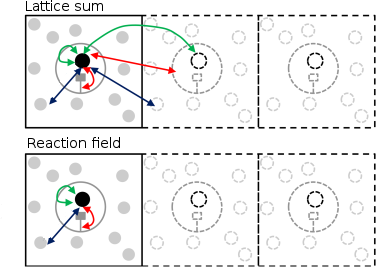
\includegraphics[width=0.4\textwidth]{figures/reif_oostenbrink.png}
    \caption{\textbf{Graphic illustration of contributions to binding free energy introduced when changing the net charge of the system.}  It is common practice to truncate Coulomb interactions beyond a certain range to reduce calculation costs and use methods such as PME~\autocite{Essmann1995a} or reaction field~\autocite{Tironi1995a} solvation models to compensate for the loss of interaction beyond the cutoff. When there is a net charge change, this leads to errors in treatment of interaction between ligand and solvent molecules beyond cutoffs and interactions with periodic copies of the system (blue arrows). Likewise, interactions between macromolecule and ligand need to be corrected (red arrows). Lastly, self interacting terms may also introduce errors when charges are removed (green arrows). Figure adapted from \textcite{Reif2013a}.}
  \label{figure:chargecorrections}
\end{figure}

\subsubsection*{Protonation state effects can be important in kinase inhibitor binding, but the scope of this problem is unknown.}
Kinases are important signaling proteins, and for a long time its been known that disregulation of some kinases can lead to cancer~\autocite{Levinson1978a,Vivanco2002a}.
%
They are a promising drug target, and many drugs have successfully been developed to inhibit kinases that are disregulated in cancer~\autocite{Baselga2006a,Garber2006a,OHare2011a}.
%
Unfortunately, intrinsic or induced mutations can lead to resistance, meaning there is a continued need for drugs to overcome resistance~\autocite{Shah2004a,Pao2005a,Garber2006a,Zhang2009a}.

Imatinib (Gleevec) is a potent inhibitor of Abl kinase~\autocite{Druker2001a}, and has shown high efficacy in patients with chronic myeloid leukemia~\autocite{OBrien2003a}.
%
At physiological \pH, it has access to multiple protonation states (\Cref{figure:imatinib-pKa})~\autocite{Szakacs2005a}.
%
Furthermore, from computation and experiment, there is evidence that there could be \pH dependent effects to the binding affinity~\autocite{Seeliger2007a,Lin2013a}.
%
The use of incorrect or inappropriate protonation states in modeling protein-ligand association can significantly degrade accuracy~\autocite{Polgar2005a,Wittayanarakul2008a}.
%
But what if there is not a single protonation state that contributes to the binding affinity?
%
With the exception of a few well-studied cases~\autocite{Dullweber2001a,Aleksandrov2007a,Czodrowski2007a,Steuber2007a,Czodrowski2007b},
the ubiquity of protonation state changes and the magnitude of their contribution to binding affinities in protein-ligand association in general is completely unknown.
%
Preliminary data (\Cref{figure:pka-kinase}) suggests that many kinase inhibitors have multiple accessible protonation states at physiological \pH.
%
We expect there are two separate effects that could be relevant:
\begin{enumerate}
 \item A significant population of mixtures of protonation states may be present.
 \item Changes in the dominant protonation state could occur upon binding.
\end{enumerate}
%
Modeling the system with a single protonation state can in either case lead to large errors.
%
As some kinase inhibitors bind with picomolar affinity to their target (corresponding to 28 $k_BT$)~\autocite{Knight2005a}, a 500-fold affinity loss (6 $k_BT$, equivalent to 2.6 log unit change in the equilibrium constant) would still maintain sub-nanomolar potency.
%
This suggests that a majority of these compounds could access multiple protonation states while still retaining a high binding affinity (\Cref{figure:pka-kinase}).
%
Neglecting the potential of sampling alternate protonation states would thus lead to large errors in predicted binding affinities.
%
Such large contributions could play a significant role in the selectivity of kinase inhibitors for their targets.
%
Therefore, it is essential to know whether these effects need to be incorporated if one wishes to use alchemical free energy calculations for the prediction of kinase inhibitor binding affinities.

\begin{figure}[H]
\centering
\begin{subfigure}{.48\textwidth}
  \centering
	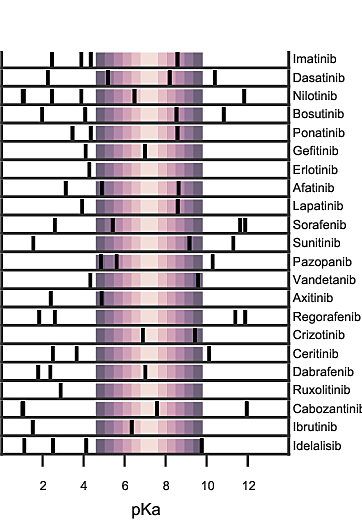
\includegraphics[width=0.8\linewidth]{figures/inhibitor-pKas.png}
	\caption{}
	\label{figure:pka-kinase}
\end{subfigure}%
\hfill{}
\begin{subfigure}{.48\textwidth}
  \centering
  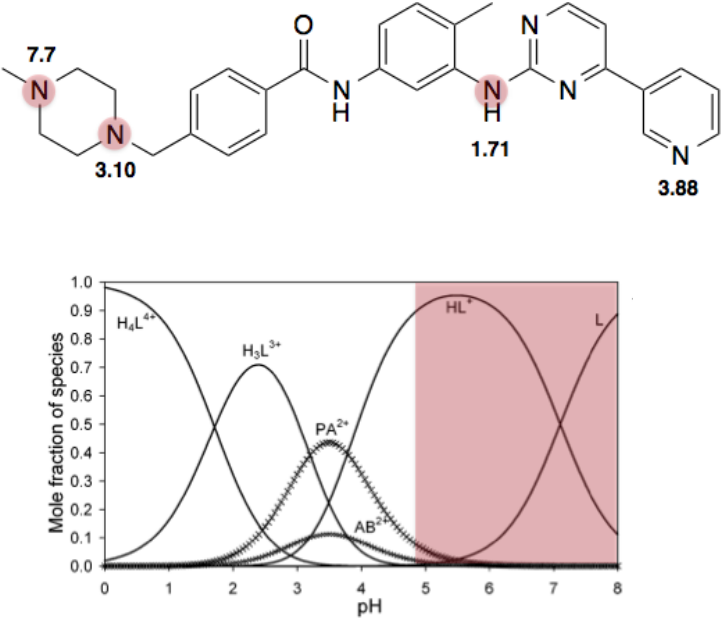
\includegraphics[width=0.9\linewidth]{figures/imatinib_image_curve.png}
  \caption{}
  \label{figure:imatinib-pKa}
\end{subfigure}
\caption{(a) \textbf{Protonation states accessible to FDA approved kinase inhibitors.}
The intracellular \pH of most tumors is around 7.2~\autocite{Griffiths1991a,Stubbs2000a}.
Colors indicate accessibility of states at \pH 7.2 within blocks of $k_BT$ units of energy, where darker means more units of $k_BT$ away from the accessible region, up until 6 $k_BT$.
Preliminary data obtained using Epik~\autocite{Shelley2007a,Greenwood2010a}.
(b) Top: The individual sites of protonation of imatinib (Gleevec) accessible with a penalty of 6 $k_BT$ under physiological conditions, highlighted in red~\autocite{Szakacs2005a}. Bottom: fraction of species of imatinib measured by titration and NMR~\autocite{Szakacs2005a}, with the red region denoting states accessible with a penalty of 6 $k_BT$ under physiological conditions.}
\label{figure:kinase-pKa}
\end{figure}


\subsubsection*{Multiple (weak) ligand binding models are required for studies of HSA and fragment based drug design.}
Most experimental tools and theoretical frameworks focus on 1:1 association of proteins and ligands, but these tools must be extended if one wishes to accurately describe binding of multiple ligands to human serum albumin (HSA), or the weak association of multiple fragments with a protein.
%
\textbf{This proposal addresses deficiencies in existing frameworks by dealing with the association of multiple ligands, as well as weak association, enabling accurate modeling of human serum albumin and protein-fragment binding.}

Because HSA controls the bioavailability of small molecules by absorbing them into the bloodstream~\autocite{Smith1985a,Jr.1995a}, it essential to understand how drugs interact with it if one wants to predict pharmacokinetics~\autocite{Smith1985a,Bannwarth1996a,Kragh-Hansen2002a,Sulkowska2002a,Zsila2011a}.
%
It binds multiple ligands simultaneously~\autocite{He1992a,Jr.1995a,Curry1998a,Ghuman2005a,Pal2013a}, making it hard to model in existing frameworks.
%
The (weak) association of multiple ligands is a significant problem in fragment based drug discovery (FBDD), that occurs because of the high concentrations used in experiments.
%
FBDD is frequently applied and has impacted the way the pharmaceutical industry and academia alike approach small molecule design~\autocite{Hajduk2007a}.
%
The association of these fragments is hard to model computationally, because of the challenges associated with modeling weak interactions~\autocite{Gilson1997a}, and the absence of modeling frameworks for multiple association.
%
Modeling deficiencies need to be addressed if free energy calculations are to be used to rationalize and predict fragment binding.
%


\section*{Research Strategy - Innovation}
\instr{Explain how your proposal differs from what others have tried.}
\subsubsection*{Reliable uncertainty estimates of isothermal titration calorimetry results by using Bayesian inference.}
If experimental results are to be used to validate theoretical models, it is essential that one accurately estimates the uncertainty of the experiment.
%
\textbf{Otherwise, it is impossible to tell whether experiment and theory differ from each other in a statistically significant way.}

The ABRF-MIRG'2 study revealed the disturbing fact that the uncertainty of ITC experiments is underestimated by several orders of magnitude by conventional analysis methods~\autocite{Myszka2003a}.
%
Panel D of \Cref{figure:abrf-mirg2} indicates a statistical uncertainty of at least 10\% in the estimation of extinction coefficients between all participants of the study, which is directly proportional to the concentration of reagents prepared by each lab.
%
The error in reagent concentrations is not correctly propagated into the estimates of binding stoichiometry, affinity and enthalpy  (Panels A, B and C of \Cref{figure:abrf-mirg2}), leading to inaccurate estimates of the uncertainty of these observables.

The underestimation of the error could have been prevented by performing adequate replicate experiments.
%
By only performing technical replicates and no repeat experiments with newly prepared reagent solutions, the true uncertainty cannot be quantified.
%
A hypothesis cannot be supported by a single experiment, and technical replicates perform but a single experiment, where only the measurement is carried out multiple times~\autocite{Vaux2012a}.

Alternatively, one can get an accurate estimate of the uncertainty by performing Bayesian inference on their experiments.
%
We propose the usage of Bayesian statistics as a means of uncertainty estimation as opposed to errors from model fit based on single or replicate experiments.
%
A Bayesian analysis of ITC experiments allows one to get more value out of single experiments, reducing resource costs.
%
This is because Bayesian inference allows prior knowledge about possible errors of reagent concentrations to be propagated into the uncertainty estimates of model parameters such as binding affinity, enthalpy and stoichiometry.
%
It thereby provides better uncertainty estimates from single experiments than standard analysis approaches, which do not propagate prior information on errors.

\thisfloatsetup{capposition=beside,
capbesideposition={center,right}}
\begin{figure}[H]
	\centering
	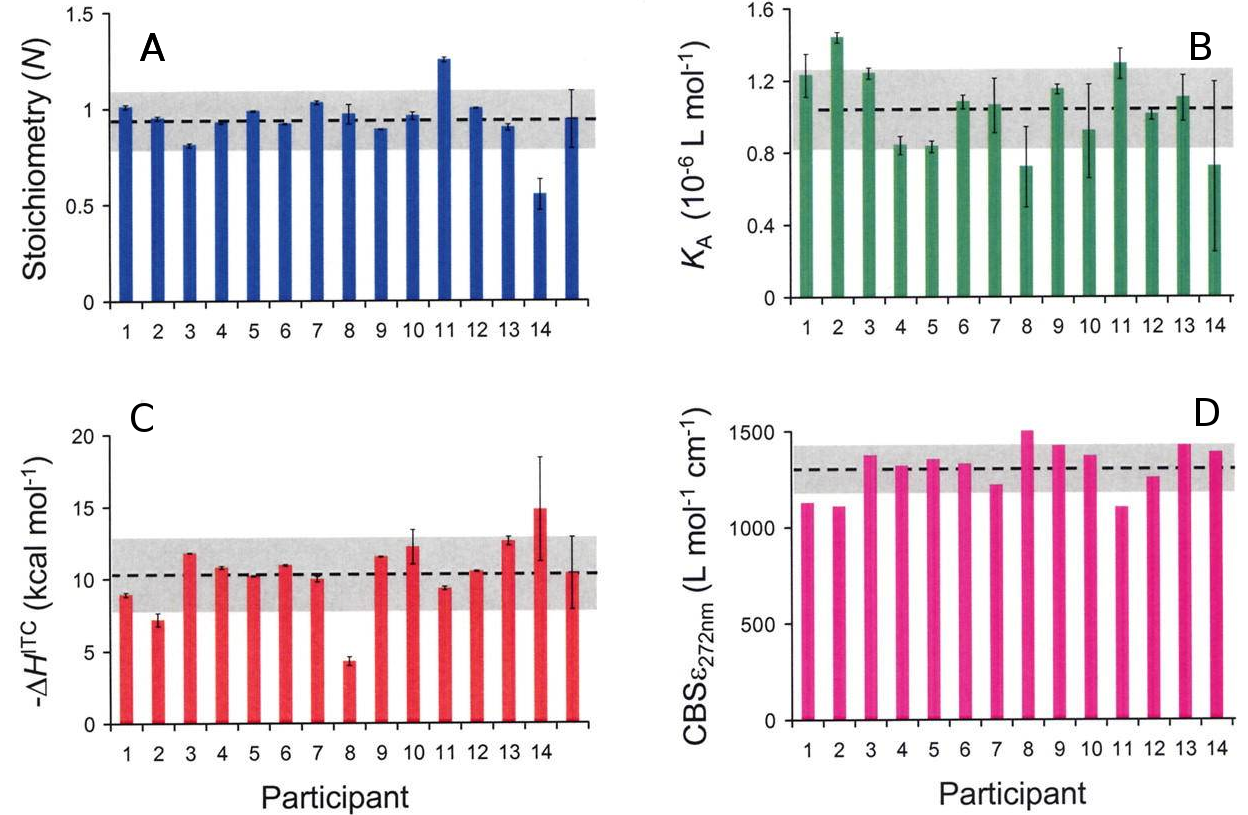
\includegraphics[width=0.49\textwidth]{figures/cbs_ca_II.PNG}
	\caption{Binding measurements of CBS to bovine carbonic anhydrase II from the ABRF-MIRG'2 study. \textbf{Independent ITC as performed by 14 labs shows individual error estimates are orders of magnitude smaller than actual experimental variation.} A: Predicted stoichiometry of binding. B: Association constant $K_\mathrm{A}$. C: enthalpic contribution to binding. D: Measured extinction coefficient of ligand CBS, as reported by the 14 participants~\autocite{Myszka2003a}. Error bars indicate the error as reported by the individual labs that were part of the study. The gray region indicates the uncertainty when taking into account all of the measurements. As can be seen, some labs underestimate the overall error by over 2 orders of magnitude. The extinction coefficient, as displayed in panel D is directly proportional to the concentration, revealing that concentration errors of around 10 percent are likely not propagated correctly into the analysis.}
	\label{figure:abrf-mirg2}
\end{figure}

\subsubsection*{Assessing proposed charge corrections in alchemical free energy calculations of charged ligands.}
Alchemical free energy calculations involving charged ligands in explicit solvent suffer from artifacts due to the treatment of the system as an infinite periodic box, and approximations in the electrostatic models~\autocite{Rocklin2013b,Muddana2014a}.
%
Several means of correcting for these artifacts have been suggested~\autocite{Reif2013a,Rocklin2013a,Lin2014a}.
%
\textbf{A quantitative comparison of these methodologies to each other and to experiment has not yet been performed, and the correctness of any of these available charge correction methods has not been established.}
%
Our work will contribute substantially to the understanding of these charge corrections by providing an experimental dataset with small and quantified uncertainty, against which models can be validated.
%
For the first time these models will be compared to each other by simulating the same system.
%
We can determine whether these methods provide consistent corrections, and at the same time the experimental dataset allows the assessment of quantitative agreement with experiment.

\subsubsection*{Quantifying unknown contributions to kinase-inhibitor binding specificity by modeling protonation state effects.}
Imatinib, a potent inhibitor of Abl kinase~\autocite{Druker2001a}, has access to multiple protonation states at physiological \pH (\Cref{figure:imatinib-pKa})~\autocite{Szakacs2005a}, and there is evidence of \pH dependent effects to the binding affinity~\autocite{Seeliger2007a,Lin2013a}.
%
The magnitude of these contributions still remains to be elucidated, and preliminary data (\Cref{figure:pka-kinase}) suggests that many other kinase inhibitors have multiple accessible protonation states at physiological \pH.
%
\textbf{This work will be the first attempt to comprehensively identify and quantify these effects for known kinase inhibitors, both experimentally and computationally.}
%
Some well studied model systems have shown that protonation state changes can contribute significantly to ligand binding affinity ~\autocite{Dullweber2001a,Aleksandrov2007a,Czodrowski2007a,Steuber2007a,Czodrowski2007b}, yet contribution of protonation state effects to binding affinities in protein-ligand association in general is completely unknown.
%
Providing the evidence that this is important for kinase inhibitors may lead to further studies into how this contributes to inhibitor selectivity, a poorly understood characteristic of many kinase inhibitors~\autocite{Knight2005a,Karaman2008a}.
%
It may also warrant the investigation of these effects in other classes of proteins, while at the same time this proposal provides the tools to perform these investigations.

\subsubsection*{Estimating free energies of multiple ligands using semi-grand canonical ensemble free energy calculations.}
Most experimental and modeling frameworks for treatment of protein-ligand binding focus on 1:1 association.
%
Conversely, to model binding of ligands to serum albumin, or to model the weak binding of fragments to a protein, one needs to model the association of multiple ligands.
%
Association of multiple ligands to a protein are not adequately treated by most analysis and modeling frameworks.
%
\textbf{This work will provide novel computational and experimental frameworks that will allow for the simulation and analysis of multiple ligand association with a single target.}
%
It also provides a solution for some of the challenges associated with modeling weak interactions~\autocite{Gilson1997a}, commonly observed in fragment binding~\autocite{Hajduk2007a}.
%
The alchemical framework that we suggest handles the association of weak ligands by sampling the overall free energy of association as a function of the number of ligands bound, without focusing on individual binding sites.
%
The model for multiple ligand association can be derived from semi-grand canonical ensemble theory~\autocite{Dill2010a}.
%
The semi-grand canonical ensemble also allows for the direct, quantitative connection between alchemical free energy calculations and ITC experiments.
%
This quantitative connection can be used both to suggest experiments that can validate the model, and to enable simulations of ITC experiments to optimize experimental design.

\section*{Research Strategy - Approach}
\instr{Approach: More specific background information. Describe in detail the experimental design and research methods to be used. Technical hurdles to be overcome should be mentioned. Alternative approaches should be given for experiments that may not be feasible. Discussion of expected or possible results and their interpretation. Best format for each specific aim: a) rationale, b) methods, c) expected results, d) alternatives. Theory aims should follow a similar structure where possible.}


\subsection*{Aim 1. Establish a correct quantitative treatment of alchemical free energy calculations for binding of charged ligands}
\subsubsection*{Rationale}
The soluble form of many drugs and endogenous small molecules is charged. Yet, retrospective studies and predictive challenges show current free energy methodology makes substantial errors in the treatment of binding by charged species~\autocite{Rocklin2013b,Muddana2014a}.
%
For explicit solvent simulations using particle mesh Ewald ---the gold standard approach to simulating solvated biomolecular systems--- a number of details of the calculation impact macroscopic observables when the total charge of the system or the overall charge density changes by removal of a charged ligand.
%
A number of approaches for explicitly solvated PME free energy calculations with charged species have been proposed, but (1) consensus, and (2) a good model system to test and to confirm theory are lacking~\autocite{Reif2013a, Rocklin2013a, Lin2014a}.

We propose using the association of small-molecule guests with high-affinity supramolecular hosts as a way to test, validate, and refine both theory and algorithms applicable to charged ligands.
%
We will use cucurbit[7]uril (CB7) as a host~\autocite{Lagona2005a}, which is known to bind a series of cations within a range of affinities spanning several orders of magnitude (\Cref{figure:host-guest})~\autocite{Cao2013a}.
%
In order to provide an experimental dataset with accurately quantified uncertainty, we will perform isothermal titration calorimetry (ITC) experiments of various guests binding to CB7.
%
We will then perform alchemical free energy calculations to evaluate the available approaches in an attempt to support or refute them.

%
ITC experiments will benefit from the high solubility of CB7.
%
CB7 is more soluble than many proteins, \SIrange[scientific-notation=false]{20}{30}{millimolar}~\autocite{Lagona2005a} in water versus \textless~\SI{1.0}{millimolar} for a small soluble protein such as RNAase Sa~\autocite{Pace2004a}.
%
This will allow us to reach higher concentrations, which will make for more tractable experiments.

The small system size provides an additional advantage for molecular dynamics simulation, since the limited degrees of freedom will make sampling more efficient and reduces computational cost.
%
Unlike biomolecules, CB7 does not undergo large-scale conformational changes and has small correlation times~\autocite{Mock1989a,Tang2011a}.

\begin{figure}[H]
\centering
\begin{subfigure}{.5\textwidth}
  \centering
  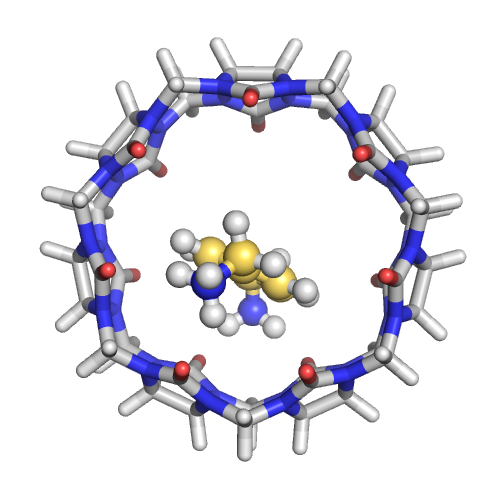
\includegraphics[width=.4\linewidth]{figures/guest11_top.png}
  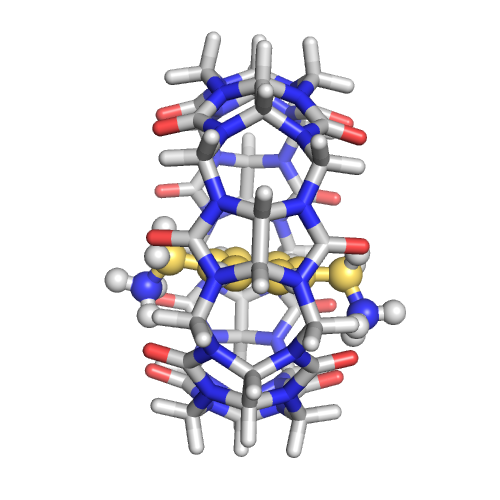
\includegraphics[width=.4\linewidth]{figures/guest11_side.png}
  \caption{A divalent guest bound to bound to the central cavity of CB7.}
  \label{fig:sub1}
\end{subfigure}%
\begin{subfigure}{.5\textwidth}
  \centering
  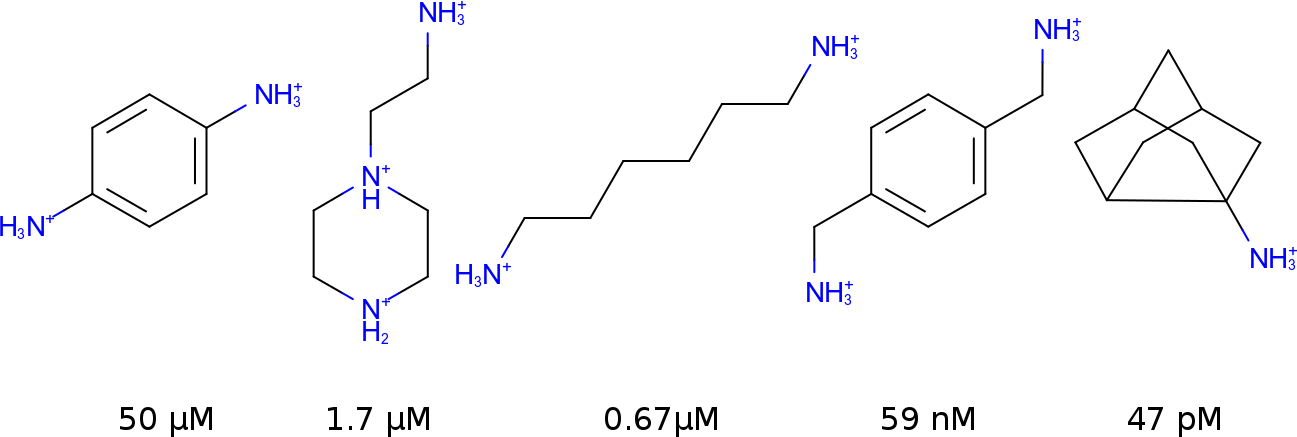
\includegraphics[width=1\linewidth]{figures/Kd_guest2.png}
  % JDC: All of the guests are scaled in weird ways making benzene rings different sizes.  Would be great to fix this at some later point, but not essential now.
  \caption{A selection of guests and their $K_d$ values from \textcite{Cao2013a}.}
  \label{fig:sub2}
\end{subfigure}
\caption{\textbf{Cucurbit[7]uril (CB7) bound to several cationic guests from \textcite{Cao2013a}}. Different guests bind to the central cavity of CB7, their affinity determined by their geometry and size. Their affinities are in a range similar to many protein-ligand complexes, though the complexes are small, with few degrees of freedom, making them excellent candidates for our study. Figure prepared using Glide docking~\autocite{Halgren2004a,Friesner2004a,Friesner2006a,Schroedinger2014a} into crystal structure pdb:QQ7~\autocite{Feng2004a}.}
\label{figure:host-guest}
\end{figure}

ITC has been shown to lead to serious underestimation of measurement error due to failure to propagate errors in the concentration of reactants~\autocite{Myszka2003a,Tellinghuisen2011a}.
%
To provide an accurate assessment of error from single experiments, we will develop a novel analysis method using Bayesian inference.
%
The framework of Bayesian inference allows for the propagation of errors throughout the experimental procedure, allowing us to accurately quantify the experimental uncertainty, thereby enabling us to clearly refute or support the various approaches to dealing with charged ligands.
%
We will consider the approaches of \textcite{Reif2013a}, \textcite{Rocklin2013a}, and \textcite{Lin2014a} for eliminating the contribution of net charge.  Each scheme mostly agrees on the source of error, but has a different way of solving the problem, as described in Subaim 1.2.
%
We will also consider the elimination of neutral salt pairs, in lieu of corrections, to evaluate the necessity of these complex schemes.


\subsubsection*{Subaim 1.1: Develop an accurate approach to quantifying experimental uncertainty in ITC using Bayesian inference.}
To test and confirm theoretical models, an accurate quantitative estimate is needed of the experimental error of the experiments that are used to validate.
%
We will develop Bayesian approaches to accurately quantify measurement uncertainty and allow for model-error propagation.
Errors in the concentration of prepared solutions are a major source of uncertainty in ITC data. Not taking these into account can lead to orders of magnitude underestimation of the uncertainty of the experiments~\autocite{Myszka2003a,Tellinghuisen2011a}.
One way to take this into account is by doing repeat experiments in which all solutions are prepared anew for each replicate, instead of technical replicates~\autocite{Vaux2012a}. This however is time and material consuming, and therefore not a popular option among most scientists.

In a Bayesian approach, we can assign prior distributions to the true concentrations of both species, allowing the uncertainty in these concentrations (tracked during solution preparation via standard propagation of error) to be used as input.
Using \textit{Markov Chain Monte Carlo} (MCMC)~\autocite{Metropolis1953a,Hastings1970a}, we can then sample from a joint posterior probability distribution of all thermodynamic parameters to estimate the actual concentration, using\textit{Bayes' rule}
%
\begin{align}
	\mathcal{P}\left(\theta | \mathcal{D} \right) \propto  \mathcal{P}(\mathcal{D} | \theta) \mathcal{P}\left(\theta\right) \quad;\quad \theta   =  \left\{ \Delta G_\mathrm{bind}, \Delta H_\mathrm{bind}, \Delta H_0, [\mathrm{X_{syr}}], [\mathrm{M_{cell}}], \sigma \right\}
\end{align}
%
where $\mathcal{P}(\mathcal{D}|\theta)$ is the likelihood of the data $\mathcal{D}$ (i.e., injections heats $q_n^\mathrm{obs}$), given the individual thermodynamic parameters $\theta$, and $\mathcal{P}(\theta)$ is a prior distribution of the set of independent thermodynamical parameters. Our posterior model contains parameters such as the binding affinity ($\Delta G_\mathrm{bind}$), the enthalpy of binding ($\Delta H_\mathrm{bind}$), an offset to incorporate mechanical and dilution effects ($\Delta H_0$),  the true reagent concentrations in the syringe ($[\mathrm{X_{syr}}]$), and in the sample cell ($[\mathrm{M_{cell}}]$), and $\sigma$, the square root of the variance of our measurements.

The simplest likelihood model of an ITC experiment consist of a series of $n$ injections, resulting in injection observed heats $q_n^\mathrm{obs}$,
%
\begin{align}
	q_n^\mathrm{obs} \sim \mathcal{N}(q_n^\mathrm{true}, \sigma^2) \quad ,
\end{align}
%
which are drawn from a normal distribution $\mathcal{N}$ with a variance of $\sigma^2$ and with the true injection heats $q_n^\mathrm{true}$ as the underlying mean. As stated by the central limit theorem (CLT), the sum of the individual power measurements, integrated to give the heat of single injections, will be normally distributed.

The methodology will allow incorporation of multiple experiments, such as calibrations, to accurately separate out heat effects due to e.g. dilution of the chemicals used or mechanical effects of the injections.

We will collect ITC data for the series of guests used by \textcite{Cao2013a} binding to CB7. Experiments will be performed using an Auto iTC-200 instrument, available at the Rockefeller University High-Throughput and Spectroscopy Resource Center (HTSRC). The experimental setup will be designed using a Python library~\autocite{vanRossum1995a} developed in house for the design of ITC experiments, and the setup will be carried out on our in house laboratory automation system using procedures generated by the library.

\subsubsubsection{Subaim 1.2: Perform a quantitative comparison of suggested correction models to experiments to establish a correct treatment of charged ligands in alchemical free energy calculations.}
We will compare several methods that correct for changes in the net charge of the system in alchemical free energy calculations~\autocite{Reif2013a,Rocklin2013a, Lin2014a}, in order to estimate which methods can provide quantitatively correct estimates of the binding affinity.
%
To do so, we will perform alchemical binding free energy calculations on the series of guests-CB7 complexes for which binding affinities were measured as part of Subaim 1.1 and compare the methods to the experimental results.

We will consider a total of four schemes that account for charged ligand binding.
%
The approach of \textcite{Reif2013a} uses a thermodynamic cycle to define a raw charging contribution to binding free energy, and tries to deconvolve the various contributions so that they can be subtracted from the total binding free energy.
%
\textcite{Rocklin2013a} suggests a numerical, as well as an analytical scheme to calculate contributions, both using Poisson-Boltzmann (PB) calculations on the protein-ligand system.
%
Then, there is the approach of \textcite{Lin2014a}, who use potential of mean force (PMF) calculations in a single simulation system with a macromolecule and ligand unbound, separating them by a large distance in explicit solvent.
%
We will also test an additional model that does not apply corrections, in which a neutral ligand:counterion pair is alchemically eliminated.


%
We will first consider whether all methods agree with each other, and the extent of the difference between their estimates.
%
Discrepancies between the results could indicate that some of the approaches are quantitatively incorrect.
%
If the various approaches agree, we can compare them in terms of computational efficiency.
%
Next, we will compare each of the approaches to the experimental data, to see whether any of them produce a quantitatively correct result.
%
The accurately quantified uncertainty of our experimental data will provide us with a means to refute or buttress the proposed correction schemes.



\subsubsection*{Expected results}
The ITC experiments performed on the CB7-guest complexes will be analyzed using our Bayesian ITC analysis method.
%
This will provide us with estimates of their binding affinity with accurately quantified uncertainty.
%
Then, we will perform alchemical binding free energy calculations, in an attempt to reproduce the experimental data.
%
We will evaluate whether each of the individual schemes produces the same answer and will estimate the difference between their estimates.
%
Next, we can compare the result obtained by each scheme to the experimental results. If their estimate falls within the range of the experimental estimate, then it supports the suggested approach.
%
Each of the methods carries an increased computational cost with them, compared to not applying corrections.
%
By applying them on the same system, we can also get an estimate on how efficient they are in costs versus improved accuracy.
%
We will then be able to recommend a methodology to use when calculating the free energy of binding for charged species.


\subsubsection*{Pitfalls and alternatives}
It is possible that all methods produce comparable results, in which case we can perform a comparison of efficiencies to determine which method is best.
%
Another potential outcome is that none of the models are able to reproduce the experimental results.
%
This could indicate problems with the force field used to simulate the systems.
%
We can use a variety of different force fields to estimate errors that are due to the force field.
%
For instance, we could compare the GAFF\autocite{Wang2004a}, GAAMP\autocite{Huang2013a}, and OPLS\autocite{Schroedinger2014b} force field models to get an estimate of the force field error.

To further estimate force field error, we could perform the same experiments and alchemical free energy calculations using a neutral guest.
%
This would leave out the contribution due to a net charge change, so that the accuracy of the force field can be assessed.
%
We may find the need to try more complicated models for our Bayesian analysis of the ITC experiments.
%
We can incorporate effects such as dilution heats, injection volume errors, and sophisticated baseline estimation to improve our estimates.

\subsection*{Aim 2. Quantify the magnitude of protonation state effects on binding}
\subsubsection*{Rationale}
Proteins and many small-molecule drugs contain titratable moieties that can change protonation state upon binding or sample mixtures of protonation states, often in a conformation-dependent manner.
%
Evidence exists that for the binding of imatinib to Abl kinase, \pH dependent effects may contribute to the binding affinity\autocite{Szakacs2005a, Seeliger2007a, Lin2013a}.
%
Our preliminary investigations suggest that the same effects will be relevant to a large number of FDA approved kinase inhibitors (\Cref{figure:pka-kinase}).
%
Kinases are important signaling proteins, and for a long time its been known that disregulation of some kinases can lead to cancer~\autocite{Levinson1978a,Vivanco2002a}.
%
They are a promising drug target, and many drugs have succesfully been developed to inhibit kinases that are disregulated in cancer ~\autocite{Baselga2006a,Garber2006a,OHare2011a}.
%
Kinase inhibitors typically have high potency~\autocite{Knight2005a}, so protonation state effects may mostly go unnoticed in standard experimental assays.
%
The usual approach in modeling ignores these effects and assumes a single protonation state for an entire system.
%
However, they form a potential pitfall when modeling, since these unknown contributions potentially lead to large errors in the binding affinity.

While detailed biophysical studies of a few specific model systems have demonstrated that these effects can contribute several kcal/mol in binding affinity~\autocite{Dullweber2001a,Aleksandrov2007a,Czodrowski2007a,Steuber2007a,Czodrowski2007b},
the ubiquity and magnitude of protonation state effects in ligand recognition in general is unknown.
%
\textbf{Our aim is to identify kinase systems where protonation state effects influence binding, and to quantify the effect of protonation state effects on the binding affinity of kinase inhibitors.}
%
We will first survey kinase-inhibitor complexes in the protein databank (PDB)~\autocite{Berman2000a} to identify complexes in which protonation state effects may play a major role.
%
To identify whether protonation state changes may have an effect on binding in these systems, we will simulate them using a Monte Carlo titration framework called MCCE~\autocite{Song2009a} which can rapidly sample the protonation states of both inhibitor and kinase subject to a constrained backbone and fixed binding mode.
%
From the populations of protonation states sampled by MCCE, we can predict which kinase-inhibitor combinations are likely to sample multiple protonation states of importance or if large population shifts are observed upon binding.
%
For systems where MCCE simulations suggest significant involvement of protonation state effects in binding, we will investigate these further using detailed alchemical free energy calculations into which we implement a dynamic protonation state sampling scheme~\autocite{Mongan2004a,Stern2007a,Nilmeier2011a}.
%
For those systems where detailed free energy calculations show kinase and ligand experience a net change in charge and for which kinase catalytic domains can be expressed in bacteria, we will use isothermal titration calorimetry (ITC) experiments~\autocite{Baker1996a,Neeb2014a} to experimentally verify and quantify the contributions of protonation state effects to binding.
%

Both MCCE and the dynamic protonation alchemical free energy calculations require that we know the \pKa of titratable sites in our small molecules.
%
While a number of tools exist to predict these, their accuracy for kinase inhibitors is uncertain.
%
We will first benchmark these tools using experimental kinase inhibitor \pKa data for FDA-approved kinase inhibitors.
%
Once a suitable tool has been identified, we will use it to generate reference \pKas for the constant-\pH free energy calculations, combining the two into a useful framework for calculating the free energy of binding.

\subsubsection*{Subaim 2.1: Benchmark small molecule \pKa prediction tools against experimental data for kinase inhibitors.}
The dynamic protonation state simulations can only capture relevant protonation if we have accurate \pKa data for the inhibitors.
%
To identify reliable tools, we will benchmark existing \pKa prediction tools using \pKa data obtained for a series of kinase inhibitors using a Sirius T3 instrument.
%
The Sirius T3 instrument provides a gold standard for giving macroscopic \pKas using a combination of electrochemical and UV-metric titrations~\autocite{Schoenherr2015a}.
%
This will help us select a tool that can adequately predict \pKa values for kinase inhibitors with similar chemical components.
%
For an efficient framework, we would like to incorporate a reliable computational \pKa prediction tool, so that we can estimate the \pKa and simulate a system using a single, straightforward procedure.
%
Among the small molecule \pKa prediction tools considered will be \textbf{MoKa}~\autocite{Milletti2007a}, \textbf{Jaguar}~\autocite{Bochevarov2013a}, and \textbf{Epik}~\autocite{Shelley2007a,Greenwood2010a}.
%
MoKa generates \pKas based on atomistic descriptors, defined by the surrounding atoms.
%
The descriptors are based on molecular interaction fields calculated using GRID~\autocite{Goodford1985a} for a library of 3D fragments, but can successfully be applied on 2D structures.
%
Schrodinger's Jaguar provides means of estimating \pKa values using quantum mechanical methods.
%
Epik uses Hammett Taft linear free energy approaches~\autocite{Perrin1981a} for predicting \pKa values.

\subsubsection*{Subaim 2.2: Survey the kinase:inhibitor cocrystal structures for possible protonation state effects in inhibitor binding.}
We will systematically explore the effects of fixed and dynamic protonation states on kinase, inhibitor, and kinase:inhibitor complexes to determine the impact of assuming protonation states are fixed or dynamic, and to dissect the effect in terms of protein-dominated, ligand-dominated, or coupled protein-ligand effects.
%
Preliminary data indicates that a number of FDA approved kinase inhibitors have \pKa values close to the physiological \pH, including imatinib~\autocite{Szakacs2005a}, (\Cref{figure:pka-kinase}).
%
We aim to quantify these contributions, in order to find out how important they are for correctly estimating the binding affinity of small molecule kinase inhibitors.
%
We will first survey kinase:inhibitor crystal structures in the PDB interactions using MCCE~\autocite{Song2009a}, which will be extended to incorporate small molecules in its calculations using \pKa prediction tools to determine the appropriate populations of small molecule protomeric states in solution.
%
MCCE calculations of kinase, inhibitor, and complex will provide populations of protonations states at intracellular pH (approximately 7.4), sampled using Monte Carlo with a restricted protein backbone but including rotamer sampling.
%
We will then select those systems that exhibit large populations of multiple protonation states or significant population shifts of binding, as all of these effects could contribute to significant error in computed binding affinities when protonation states are assumed to be static.
%
On these systems, we will quantify the effect of protonation state changes on the binding free energy and further dissect its origin.

\subsubsection*{Subaim 2.3: Dissect the determinants and impact of protonation state effects on binding affinity through free energy calculations and ITC experiments.}
We expect that protonation state effects contribute significantly to binding affinity of the kinase-inhibitor combinations identified in the previous aim.
%
To quantify the magnitude of these effects---as well as determine their origin---we will use alchemical free energy calculations, a reliable standard for calculating binding affinities~\autocite{Fujitani2005a,Deng2006a,Wang2015a}, in which we additional implement a dynamic treatment of protonation states for a constant external pH~\autocite{Mongan2004a,Stern2007a,Nilmeier2011a}.
%
By allowing the dynamic protonation states for kinase, inhibitor, both, and neither, we will be able to both quantify the magnitude of dynamic protonation state effects and determine the primary origin of these effects.
%
The calculations will be performed using OpenMM~\autocite{Eastman2013a} and Yank~\autocite{Chodera2015a}.
%
The dynamic protonation state sampling scheme, also known as constant-\pH, allows the distribution of protons in the system to change, at a constant chemical potential of protons $\mu_{H^+}$,
\begin{align}
 \text{p}\mathrm{H} = -\log_{10}\left( a_{\mathrm{H}^+} \right) = -\log_{10}\left( \exp\left(\frac{\mu_{\mathrm{H}^+} -\mu_{\mathrm{H}^+}^\ominus}{RT}\right)\right) \approx -\log_{10}\left( [\mathrm{H}^+] \right) \quad,
\end{align}
%
where $a_{\mathrm{H}^+}$ is the activity coefficient of the protons, the superscript $\ominus$ indicates a thermodynamic standard state, $R$ is the molar gas constant and $T$ is the absolute temperature.
%
Protonation and deprotonation events are sampled using a Monte Carlo (MC) method, using the free energy of proton transfer, calculated from the electrostatic interactions, as an acceptance criterion.
%
The free energy of proton transfer depends on the reference \pKa value, as obtained from our \pKa survey, which is why we need an accurate estimate for these reference values to quantify contributions from our simulations.
%

For systems in which the kinase can be expressed in bacteria and the alchemical free energy calculations with dynamic protonation states indicate there will be a net change in charge for kinase and inhibitor upon binding, we will use ITC experiments that are able to dissect out the binding affinities of different protonation species.
%
Changes in protonation states will lead to an enthalpic contribution/penalty to the binding affinity.
%
By performing ITC experiments at the same pH using buffers with different ionization enthalpies, one is able to dissect the contribution of each protonation state to the binding affinity~\autocite{Baker1996a,Neeb2014a}.
%
To analyze these experiments, we will extend our Bayesian ITC methods to model the different experiments together to provide correlated uncertainty estimates.

\subsubsection*{Expected results}
Our initial survey with MCCE will allow us to estimate the prevalence of protonation state effects on binding of small molecule kinase inhibitors.
%
We can then quantify the magnitude by which protonation state effects contribute to the binding affinity.
%
Constant-\pH alchemical binding free energy calculations should provide us with accurate estimates, as long as we can accurately predict small molecule \pKas.
%
At the same time, we can validate these results by performing ITC experiments of these kinases-inhibitor combinations.
%
This knowledge can be used to determine whether these effects play a significant role in the selectivity of kinase inhibitors for their targets.
%
If the contribution appears to make no significant difference, we will have ruled out the need to use more expensive theoretical methods and more experimental resources.
%
We will also have developed a framework that will enable future evaluation of these effects, in systems for which experiments have not been carried out to determine the presence of these effects.


\subsubsection*{Pitfalls and alternatives}
In the case that our computational estimates of the protonation state contributions differ from our experimental estimates, this could implicate other effects have not been incorporated into our simulation.
%
For instance, the conformational states of the protein considered for our free energy calculations might need to be expanded.
%
We could use techniques such as Markov state models (MSM)~\autocite{Prinz2011a} to determine the important metastable states of kinase systems and use this knowledge to enhance our free energy calculations.
%
There could also be a problem with the predicted \pKa values.
%
In case we cannot obtain reasonable \pKa estimates, we may attempt to measure an effective \pKa experimentally from our ITC experiments.
%
Unfortunately, we can only measure exchanges between buffer and the protein or ligand, so we will need to model an effective \pKa based on this.
%
In the case that there is disagreement with experiment because of force field errors, we can perform experiments and simulations on systems where protonation state changes are not expected to occur, in order to evaluate the magnitude of this error.
%
We may also find that the charge corrections illuminated in Aim 1 are required for accuracy of dynamic protonation state calculations, so we could evaluate this if the results seem to require it.
%
Additional verification using host-guest complexes where the host or guest experience protonation state effects can be employed as needed.

\subsection*{Aim 3. Develop a framework for alchemical free energy calculations to describe weak association and cooperative ligand binding.}
\subsubsection*{Rationale}
Weak binding and association of multiple ligands to proteins are ubiquitous interactions in biological and pharmaceutically relevant systems.
%
It is particularly common when using drug discovery approaches such as fragment-based ligand design, where concentrations are scaled up to detect weak binding signals, often resulting in multiple associating fragments.
%
Most available free energy calculation frameworks focus on 1:1 binding interactions, and are not suited for calculating free energies of an arbitrary number of ligands.
%
\textbf{We will overcome deficiencies in current frameworks with a new framework that can provide predictions for ligands binding multiple times to a single macromolecule.}
%
Our proposed framework will create an alchemical ladder from $0 \ldots N_\mathrm{max}$ ligands, and can provide a description of binding by using a semi-grand canonical ensemble methodology~\autocite{Kofke1988a,Kofke1999a,Lynch2000a}.
%
We can establish a quantitative connection between these semi-grand canonical alchemical free energy calculations and ITC experiments on these systems.
%
The parameters obtained from our alchemical free energy calculations will allow us to simulate ITC experiments directly.
%
Consequently, we can use ITC experiments as a means to validate the alchemical binding free energy predictions.
%
To do so, our Bayesian framework for ITC experiments will be extended to include models of multiple binding sites.
%

As a model system, we will study the binding of several nonsteroidal anti-inflammatory drugs (NSAIDs) known to bind the pharmacologically relevant protein human serum albumin (HSA) (\Cref{figure:hsa})~\autocite{Zsila2011a}.
%
It is a protein with multiple binding sites that bind a wide variety of ligands~\autocite{He1992a,Kragh-Hansen2002a,Sulkowska2002a}.
%
Because of its ability to bind many small molecules, it is of great importance to pharmacokinetics~\autocite{Metcalfe2010a}.
%
Its high solubility makes it easy to reach the concentrations required for ITC experiments~\autocite{Jr.1995a}.
%
Many of the compounds that bind to HSA are commercially available~\autocite{Zsila2011a}.
%
The NSAIDs selected by us for this study (\Cref{figure:hsa-compounds}) are commercially available in hydrate or soluble salt forms, making them suitable for ITC experiments as well.

% \thisfloatsetup{capposition=beside,capbesideposition={center,right}}
\begin{figure}[H]
\centering
\begin{subfigure}{.49\textwidth}
	\centering
	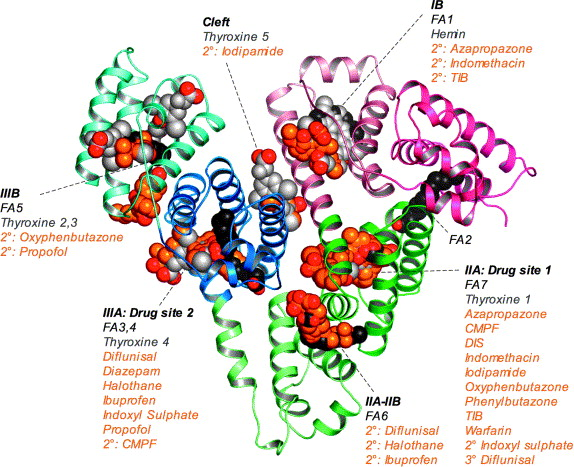
\includegraphics[width=0.9\linewidth]{figures/hsa_fig7_ghuman2005.jpg}
	\caption{
      }
	\label{figure:albumin}
	\end{subfigure}
	\hfill{}
 	\begin{subfigure}{.49\textwidth}
	  \centering
	  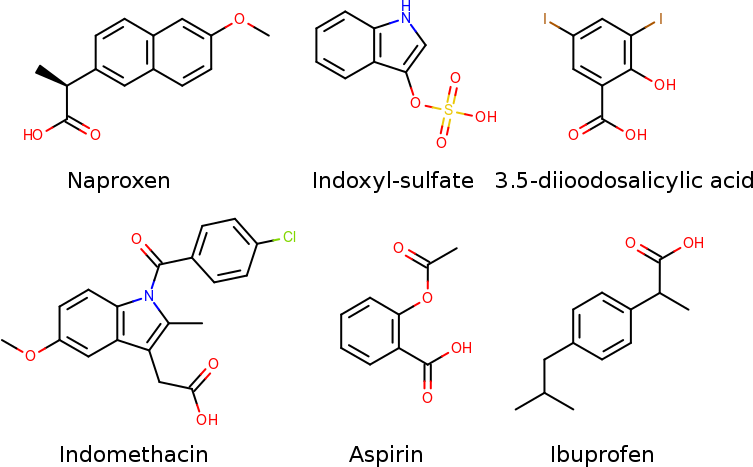
\includegraphics[width=0.9\linewidth]{figures/hsa_compounds.png}
	  \caption{}
	  \label{figure:hsa-compounds}
 	\end{subfigure}
\caption{(a) \textbf{Summary of the ligand-binding capability of Human serum albumin structural studies.} Ligands are depicted in space-filling representation; oxygen atoms are colored red; all other atoms in fatty acids (myristic acid), other endogenous ligands (hemin, thyroxin) and drugs are coloured dark-gray, light gray and orange, respectively. Because of the many small molecule interactions of HSA, it is expected to be of great importance to the bioavailability of small molecules~\autocite{Metcalfe2010a}. Its binding sites are asymmetric~\autocite{He1992a, Curry1998a} and one expects there to be a difference in binding affinity of a ligand for each site~\autocite{Sudlow1976a}. \Cref{figure:albumin} depicts the various binding sides of HSA, and shows how diverse the structure of each binding site is. It is known to bind several drugs~\autocite{SJOeHOLM1979a,Bannwarth1996a,Sulkowska2002a,Ghuman2005a,Perez2007a,Zsila2011a}, as well as dietary supplements~\autocite{Pal2013a}. It is also essential for the bioavailability of endogenous small molecules such as hormones~\autocite{Pardridge1986a}, and toxins such as cardiac glycosides~\autocite{Smith1985a}. From Figure 7 of~\autocite{Ghuman2005a}. (b) A series of commercially available NSAIDS that bind to human serum albumin, which will be used for this study~\autocite{Zsila2011a}.}
\label{figure:hsa}
\end{figure}

\subsubsection*{Subaim 3.1: Extend alchemical free energy calculations to simulate multiple ligand binding.}
Since current alchemical free energy calculation frameworks focus mostly on 1:1 association, we will need to extend available frameworks to incorporate multiple ligand binding.
%
We will build upon the existing Yank framework~\autocite{Chodera2015a} for alchemical free energy calculations to include the potential for multiple (possibly weak) binding events using a semi-grand canonical ensemble formalism.
%
Our extension allows the calculation of the free energy of the different states of a protein-multiligand complex by using an alchemical ladder that allows for binding of of 0, 1, $\dots$, $N_\mathrm{max}$ ligands.
%
As a first application of the framework we will study the binding of NSAIDs (\Cref{figure:hsa-compounds}) to HSA.
%
The compounds we have selected are known to bind to multiple sites on HSA~\autocite{Zsila2011a}, and are soluble enough to perform ITC experiments for validation of the simulation results.
%

To calculate the free energy of binding for multiple ligands, we employ semi-grand canonical ensemble theory.
%
In the semi-grand canonical ensemble (constant $\mu, N_R, p, T)$, the number of ligand molecules is allowed to vary between 0 and $N_{max}$ , and the number of receptor ($R$) molecules $N_R$ is fixed.
%
The pressure, $p$, and temperature, $T$, are also fixed. The free energy of observing $n$ ligand molecules is,
\begin{align}
 g_n = \ln \int \dif x_1 \dots \dif x_n \dif x_R \, e^{-u_n(x_1,\dots,x_n)} \quad,
\end{align}
%
where  $u_n(x_1,\ldots,x_n,x_R) \equiv \beta U_n(x_1,\ldots,x_n,x_R) + \beta p V(x)$ is the \textit{reduced} potential energy, based on the coordinates of $n$ ligand molecules and the receptor, $\beta$ is the inverse temperature, defined as $1/k_BT$, and $V(x)$ is the instantaneous volume of the simulation cell. Similarly, we can also derive the enthalpy associated with binding of $n$ ligands, $h_n$.

By knowing the free energies of each occupation state, we can estimate the bound concentrations for a given concentration of receptor $[\mathrm{R}]$ and ligand $[\mathrm{L}]$ from simulation.
%
The term in the logarithm can be substituted by what is known as the binding polynomial, $Q$
%
\begin{align}
 Q = 1 + K_1[\mathrm{L}] + K_1K_2[\mathrm{L}]^2 + \cdots + \left(\prod\limits_{i=1}^{n} K_i\right) [\mathrm{L}]^n = 1 + \sum\limits_{l=1}^n \left(\prod\limits_{i=1}^{l} K_l\right)[\mathrm{L}]^l \quad,
 \label{equation:bindingpolynomial}
\end{align}
which is also equivalent to the partition function of the system~\autocite{Dill2010a}.
%
In this equation, $K_n$ are the stoichiometric association constants, not site constants (see also \Cref{figure:semi-grand}) meaning we do not define a specific site.
%
They are obtained by taking the exponent of the free energy difference between binding of consecutive numbers of ligands
\begin{align}
K_{n+1} = \frac{[\mathrm{RL}_{n+1}]}{[\mathrm{RL}_n][\mathrm{L}]} = e^{-(g_{n+1}-g_n)} ; g_{n+1} - g_n = \ln (K_{n+1})^{-1}
\label{eq:K_eq}
\end{align}
%
The form of the equation gives us an additional benefit of modeling weak association, where we can evaluate a free energy for a number of ligands associating, even without a strongly defined binding site.

From the estimated enthalpy and association constants we can simulate an ITC experiment.
%
The heat of injection $q_m$ is a function of the enthalpy change $\Delta h_m$, cell volume $V_0$ and the change in a complex concentrations $[\mathrm{PL_n}]$ of one receptor bound to $n$ ligands
%
\begin{align}
 q_m = \sum \limits_{n=0}^{N_\mathrm{max}} q_m^{(n)} = \sum \limits_{n=0}^{N_\mathrm{max}} V_0 \Delta h_m^{(n)} \left( [\mathrm{PL}_n]_m - [\mathrm{PL}_n]_{m-1} \right) \quad. \label{equation:liberated-heat}
\end{align}
%
For a given receptor and ligand concentration, all of these properties are obtainable from free energy calculations.
%
This allows us to establish a quantitative connection with ITC experiments.

\thisfloatsetup{capposition=beside,capbesideposition={center,right}}
\begin{figure}[H]
  \centering
  \fbox{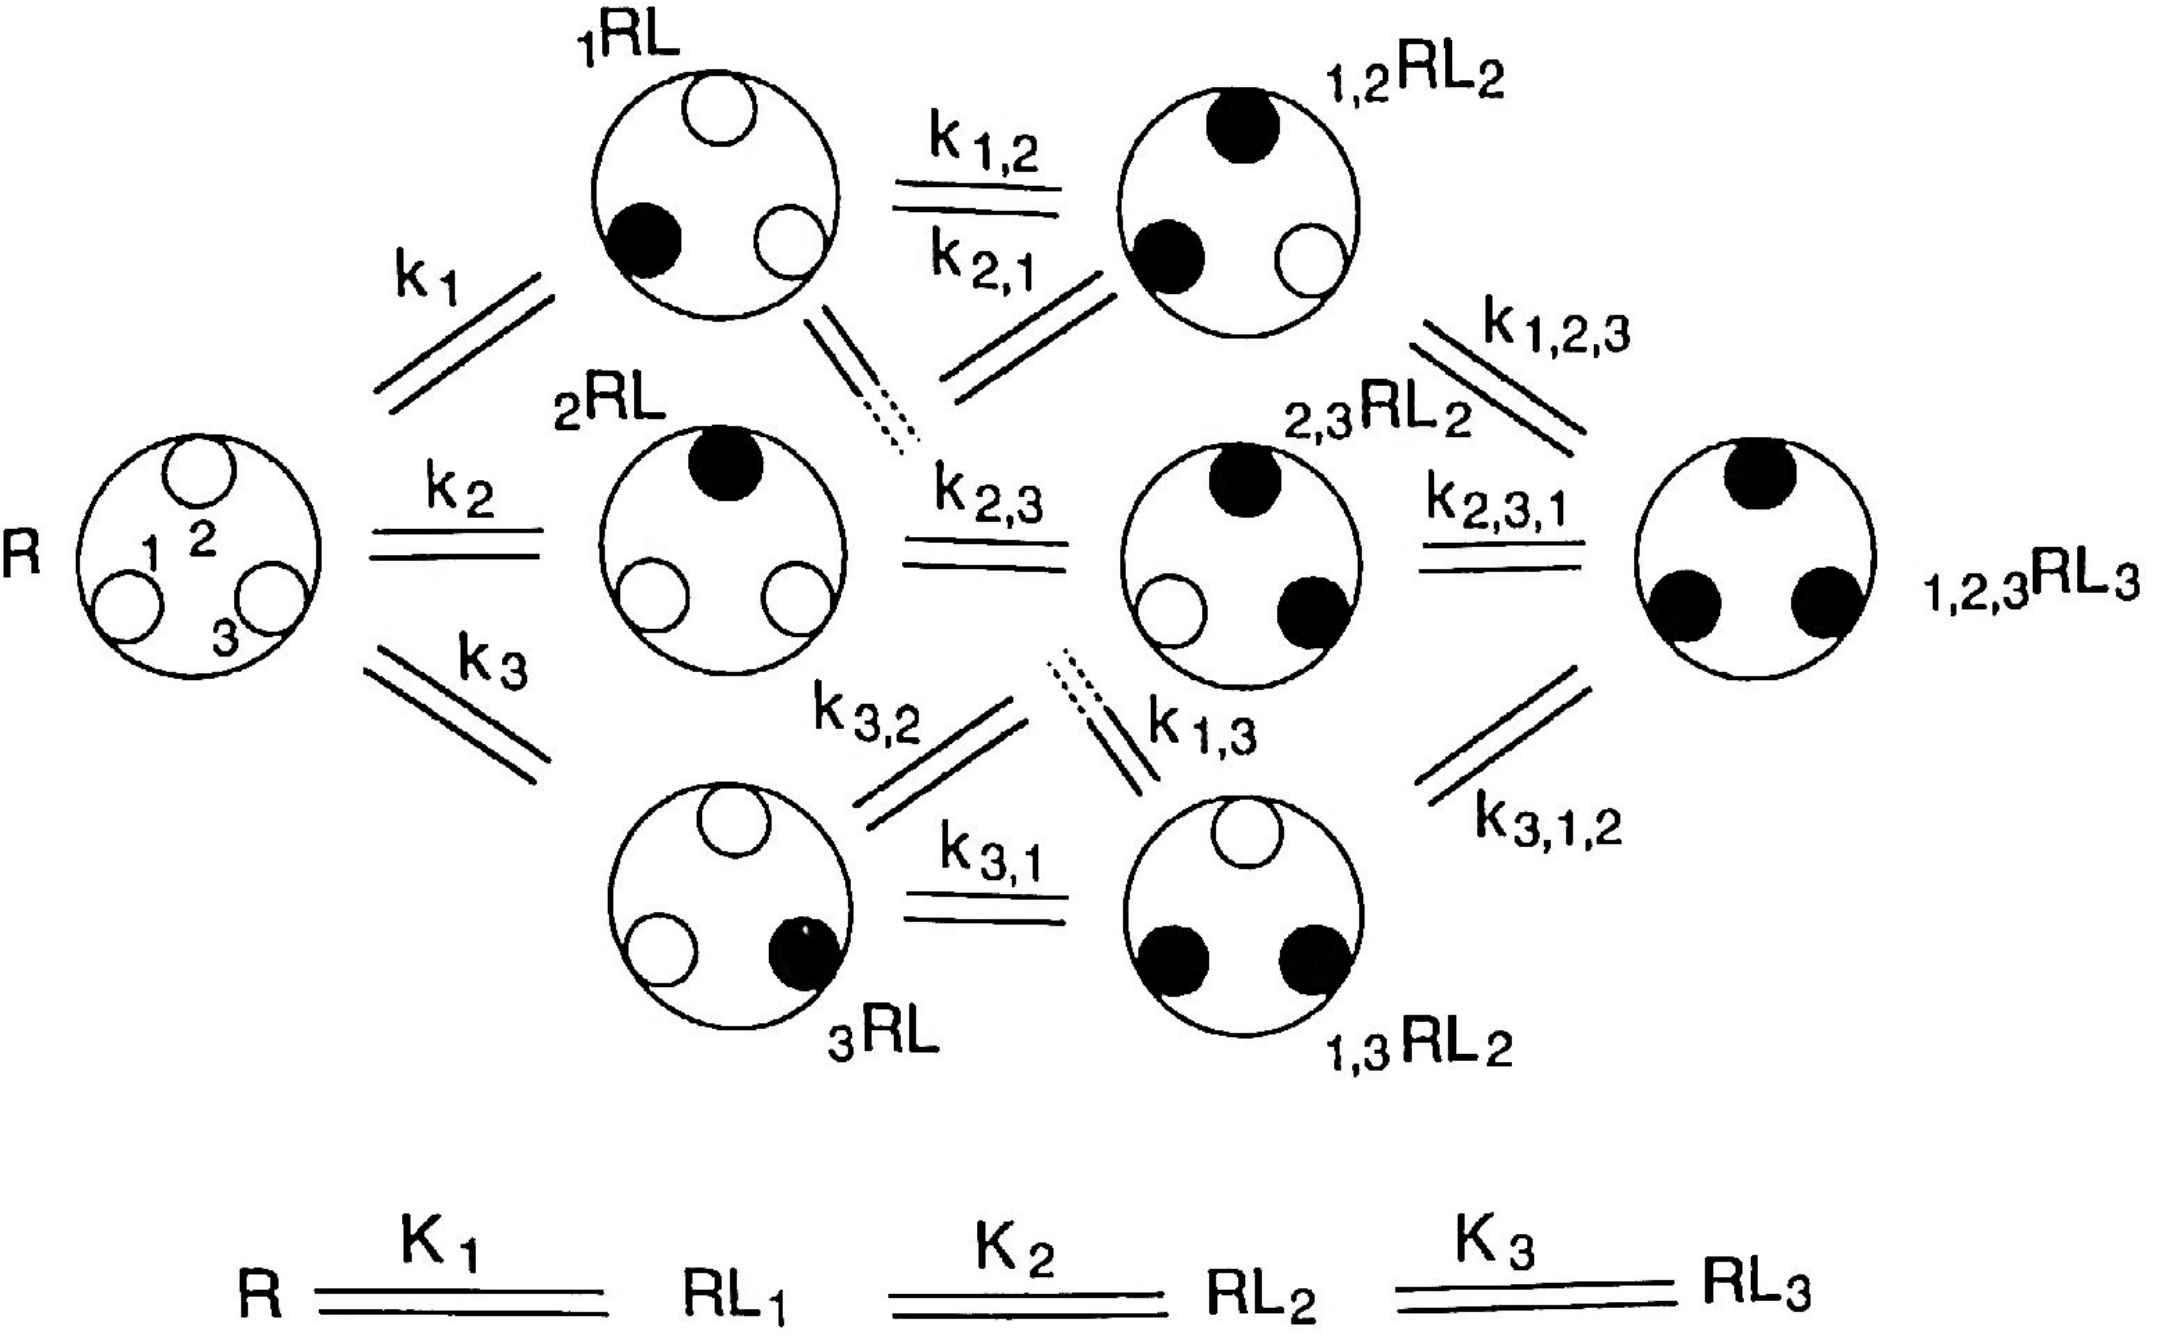
\includegraphics[width=0.4\textwidth]{figures/binding_sites2.png}}
  \caption{\textbf{In the semi-grand canonical ensemble, we consider the association of 0 up to $N_\mathrm{max}$ ligands to a protein.} By using alchemical perturbations, they can be inserted without pushing the system away from equilibrium. Rather than using site specific constants ($k$), for which specific binding sites need to be defined, we calculate the free energy of associating additional ligands to the protein by using binding polynomials of the stoichiometric binding constants $K_i$ (\Cref{equation:bindingpolynomial}). This will also allow us to calculate a free energy for weak associating ligands. Figure adapted from \textcite{Klotz1997a}. }
  \label{figure:semi-grand}
\end{figure}

\subsubsection*{Subaim 3.2: Validate computational predictions by applying Bayesian model selection on ITC  experiments of HSA and a series of NSAIDs.}
In order to validate the results obtained from free energy calculations, we will perform complementary ITC experiments on human serum albumin (HSA).
%
To design the ITC experiments, we can use the parameters obtained from the free energy calculations to simulate an ITC experiment.
%
This will allow us to find an experimental setup that can provide us with maximal information on the different binding constants.
%
We will be extending our Bayesian ITC framework, so that we can perform an adequate analysis.
%
Current ITC analysis tools are too limited in terms of their model descriptions, nor do they provide accurate uncertainty estimates due to lack of error propagation.
%
Tools like Origin~\autocite{MicroCal2004a} and NanoAnalyze~\autocite{NanoAnalyze2014a}, conventional ITC analysis software packages, uses cooperativity parameters $n_i$ to describe multiple binding sites up to a maximum of two.
%
This is too primitive to actually describe multiple binding events~\autocite{Klotz1997a}.
%
Furthermore, errors in the concentrations of the reagent solutions are not propagated, directly influencing the value of the estimated stoichiometry.
%
More advanced tools such as SEDPHAT additionally uses terms describing ``incompetent fractions'' of experimental components~\autocite{Houtman2007a,Zhao2015b} and can deal with up to 3 sites.
%
Unlike a Bayesian analysis, it does not propagate errors from the experimental procedure and just provides a ``fudge factor'' to improve the quality of the fit.
%
We will extend our Bayesian analysis tools with the capacity to use binding polynomials (\Cref{equation:bindingpolynomial}) to estimate the binding affinity and provide accurate uncertainty estimates.
%
It will be able to propagate errors in the reagent concentrations of the prepared solutions, unlike the non-Bayesian models.
%
Additionally, the binding polynomial will not be limited to necessarily 2, or 3 sites.
%
It can be extended to incorporate as many ligands as needed.
%
The number of parameters necessary can be selected by using Bayesian model selection techniques such as reversible jump Markov chain Monte Carlo (RJMCMC)~\autocite{Green1995a}.

\subsubsection*{Expected results}
The newly developed free energy calculation framework will allow us to estimate the free energy of an arbitrary number of ligands binding to a protein.
%
From these free energies, we can estimate stoichiometric binding constants, which will allow us to calculate complex concentrations for a given receptor and ligand concentration.
%
Our method will be applied on HSA, a pharmacologically relevant target, to predict the binding affinity of a series of NSAIDs.
%
The information obtained information can then be used to simulate ITC experiments of multiple ligands binding to HSA at the same time, binding to multiple sites.
%
If these estimates are correct, this will enable the design of experiments that provide more information on binding by reducing the uncertainty.
%
We can also use our Bayesian ITC analysis methodology to experimentally measure binding affinities to HSA as a means of validation of the calculations.
%
The experiments will yield credible intervals for each of the terms in the binding polynomial, with increasing uncertainty for the higher order terms.
%
The number of terms that we can fit will be limited by this uncertainty, and we can use Bayesian model selection to estimate the number of parameters to fit.
%
Using our experimental results, we can confirm whether our computational predictions fall within the experimental uncertainty.

\subsubsection*{Pitfalls and alternatives}
It is possible that our simulations will not sample many different stoichiometries, if it is unfavorable to add more ligands.
%
If that is the case, we will explore methods that drive the simulation to sample more states of the system.
%
Otherwise, our estimates of the free energy of binding will be poorly converged.
%
Higher order binding terms in the polynomial will have increased uncertainty, which will limit our ability to estimate binding free energies of accurately.
%
In order to improve the information gain, we can explore various ways of performing Bayesian experimental design.
%
This should allow us to decrease the uncertainty in the estimates.
%
We can also explore the use of alternative model systems, such as host guest systems.
%
Some hosts with larger cavities can bind multiple ligands, with their tractability making them attractive model systems.
%
Also, some hosts themselves can associate with higher stoichiometry to a solute~\autocite{Armstrong1986a}.

\section*{Conclusion}
The aims of this proposal contribute to the limited set of tools available to deal with protein-ligand interactions in special, but not rare, cases where conventional tools provide no implementation of existing theoretical frameworks. Using Bayesian methodology will provide reliable uncertainty estimates on experimental data, which in turn will enable the distinction between theoretical model errors and experimental errors.

% refs
\setlength{\emergencystretch}{1em}
\printbibliography

\end{document}
